\chapter{Computational Study}

This chapter presents our computational study and is structured as follows: 
Section \ref{sec:data} describes the data our experiments are conducted on.
Section \ref{sec:samplesize} examines how different samples sizes used for training affect the test error.
In Section \ref{sec:hpo}, we optimize model hyperparameters and seek to get better intuition when for parameter configuration by analyzing parameters considered for our optimization.
Last but not least, section \ref{sec:noise} demonstrates how noise affects predictive performance of our models.

\section{Data exploration}\label{sec:data}
The available data set is provided by \cite{Hildebrandt2020_EAT} who created a high-dimensional data model with the RMDP instances originally used in \cite{UlmerRMDP}. It comprises 850.469 samples, 23.341 unique customer locations, a delivery fleet of 15 vehicles and 15 unique restaurant locations. The temporal and spatial distribution of the orders is depicted in figure \ref{fig:dists}. 
\begin{figure}[h]
	\centering
	\subfigure[Request arrival time distribution]{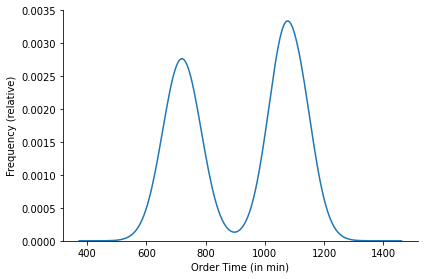
\includegraphics[width=0.49\linewidth]{../Implementation/DataDescription/order_time_dist.png}}
	\subfigure[Spatial distributions]{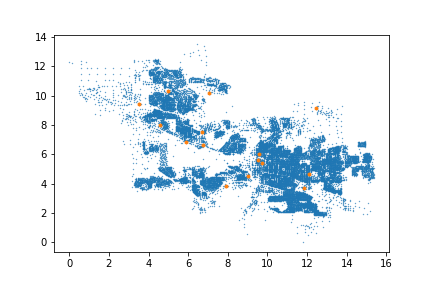
\includegraphics[width=0.49\linewidth]{../Implementation/DataDescription/spatial_dist.png}}
	\caption{Spatial and temporal distributions}
	\label{fig:dists}
\end{figure}

Panel (a) of figure \ref{fig:dists} shows the order behaviour of customers. The x-axis denotes the day time in minutes, the y-axis denotes the relative frequency of incoming customer orders for a given day time on the y-axis. We can observe that the order time behaviour across all customers follows a bimodal gaussian distribution. The order frequency peaks at around 12:00 a.m (roughly 700 minutes of day time) and again around 6.00 p.m (roughly 1100 minutes of day time). This indicates that the probability of an order taking place during lunch or dinner time is relatively high.  
Panel (b) of figure \ref{fig:dists} shows the spatial distribution of customer and restaurant locations. The x-axis depicts the  

\begin{figure}[h]
	\centering
	\subfigure[Delivery delay distribution]{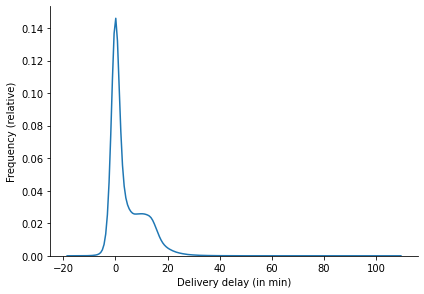
\includegraphics[width=0.49\linewidth]{../Implementation/DataDescription/delivery_delay.png}}
	\subfigure[Meal preparation time distribution]{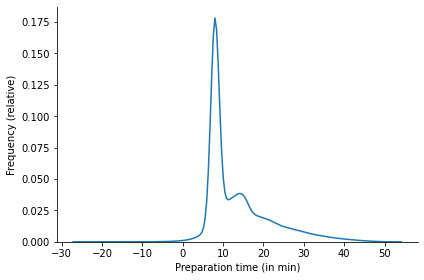
\includegraphics[width=0.49\linewidth]{../Implementation/DataDescription/prep_time.png}}
	\caption{Spatial and temporal distributions}
	\label{fig:prepdelay}
\end{figure}
Panel (a) of figure \ref{fig:prepdelay} shows the distribution of delivery delay times in minutes for all requests in the data. The delivery dela is here defined as the difference between actual and the expected time of arrival based on PoM. First, we observe that roughly 14-15\% of the requests in our data are delivered on time. Negative values for the delivery delay on the plot indicate that a rather tiny amount of orders happens to be delivered earlier than expected. However, we are most interested in the orders that are actually delivered later than expected. We observe that a non-trivial amount of orders is delivered with a delay of up to 20 minutes. As we will later show, arrival time estimation via supervised learning is a vastly better option compared to planning on means.
Since arrival times are impacted by uncertainty in meal preparation times, we take a look at their distribution in our data as well. In panel (b) of figure \ref{fig:prepdelay}, we observe that roughly a fifth of the orders had a preparation time of around 10 minutes. However, a non-trivial amount of orders seem to have quite longer preparation times ranging from 15 to less than 40 minutes. 

\section{Experiment: Different Sample Sizes}\label{sec:samplesize}

This section compares how a difference sample size impact the test error for each possible combination of models and datasets. With this experiment, we intend to examine how different sizes in training data affect the test error for the respective combination. Since less samples in the training data corresponds to lower training times, we use the results of this experiment for the subsequent hyperparameter optimization and the noise analysis to speed our experimental procedure up. For our linear model and the considered ensembles, we consider 100 training runs with every run corresponding to a sample subset size $ \{2000, 4000, \dots, 200.000\} $. For each model, we set the parameters manually since we did not conduct hyperparameter optimization yet. 

\begin{figure}[h]
	\centering
	\subfigure[For GBDT]{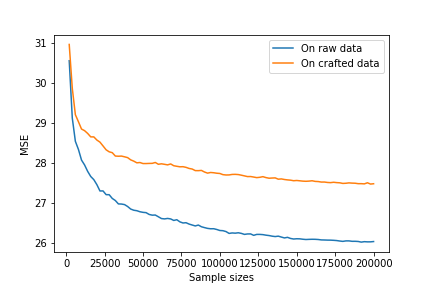
\includegraphics[width=0.49\linewidth]{../Implementation/SampleSize/GBDT_SampleSizes.png}}
	\subfigure[For Random Forest]{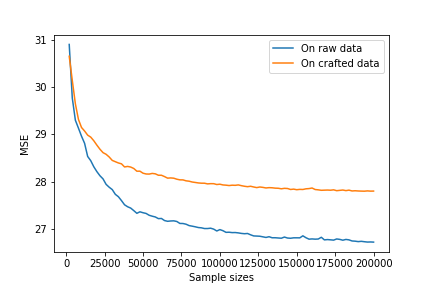
\includegraphics[width=0.49\linewidth]{../Implementation/SampleSize/RF_SampleSizes.png}}
	\subfigure[For Linear Regression]{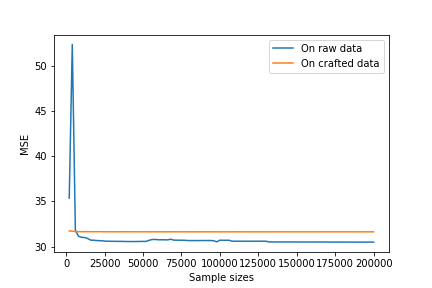
\includegraphics[width=0.49\linewidth]{../Implementation/SampleSize/LR_SampleSizes.png}}
	\caption{MSE for different sample sizes}
	\label{fig:convergences}
\end{figure}

[TODO: Explain results]
\section{Experiment: Hyperparameter Optimization}\label{sec:hpo}
This section presents the hyperparameter optimization (HPO) experiments conducted for GBDT and Random Forest.
We use \textit{Optuna}, a popular HPO framework proposed and designed by \cite{akiba2019optuna}, to conduct our HPO experiments. 
\textit{Optuna} provides a simple implementation design that allows us to analyze several parameters of choice from different points of view. 
The optimizations were conducted on both the crafted data set and the raw data set. 
Concretely, we will proceed as follows: First, we will present the hyperparameters we decided to include in the HPO to then in turn present the optimal hyperparameter values resulting from the experiment and explore the predictive power of different parametrizations. 
For every GBDT and RF experiment instance, the hyperparameters will be sampled via the \textbf{C}ovariance \textbf{M}atrix \textbf{A}daption \textbf{E}volution \textbf{S}trategy, or in short \textbf{CMA-ES}. 
\textit{CMA-ES} follows a simple principle: The probability of samples from previously succesful optimization steps being drawn again is positively correlated to the contribution of those samples to the objective. For further information on \textit{CMA-ES}, the reader is referred to \cite{hansen2016cma}. 
To speed up the optimization process, we use the \textit{Optuna}-implementation of the \textit{Hyperband Pruner} presented in \cite{li2018hyperband} and furthermore use only 200.000 of our samples since the models begin to converge at this subset size as shown in section \ref{sec:samplesize}. By that, we hope to get a fine-tuned model that maximizes prediction quality on one hand, and intuition for suitable parametrizations on the other hand.
In the next step, we will use the \textit{optuna} implementation of the \textit{fANOVA} evaluation algorithm presented in \cite{fANOVA} to determine hyperparameter importances. 
In short, \textit{fANOVA} calculates feature importances by fitting a random forest regression model to the optimal parameter configuration that results of the HPO with which it aims to predict the corresponding objective value. The relative importances provide information about the parameter variances. A higher value is associated with a higher variance, meaning that a change of the parameter setting will have a greater impact on the prediction performance compared to parameters of low relative importance. Thereby, we can assess which parameters impact the model significantly and which parameters are less significant, and especially how the importances differ for the two data sets. For each parameter importance prediction, we set the number of estimators in \textit{fANOVA} to 1000.
\subsection{GBDT}

In this subsection, we will conduct HPO experiments for GBDTs on both datasets. 
For GBDT, we decided to optimize following parameters and set the search spaces for each of them as follows:
\begin{description}[font=$\bullet$\scshape\bfseries]
	\item $ \text{learning\_rate} \in [0.01, 0.05] $  in steps of 0.001.
	\item $ \text{max\_depth} \in [5, 100] $ in steps of 0.001.
	\item $ \text{feature\_fraction} \in [0.1, 1.0] $ in steps of 0.01.
	\item $ \text{feature\_fraction\_bynode} \in [0.3, 1.0] $ in steps of 0.01
	\item $ \text{num\_leaves} \in [20, 300] $ in steps of 1
	\item $ \text{min\_child\_samples} \in [10, 400] $ in steps of 1.
	\item $ \text{subsample\_freq} \in [1, 10] $ in steps of 1.
	\item $ \text{subsample} \in [0.3, 1.0] $ in steps of 0.01.
\end{description}
Besides the parameters considered for optimization, we set the number of estimators for one iteration in GBDT to 1000 and enable early stopping with a patience of 20. Our selection of parameter search spaces is the result of trial-and-error since machine learning problems are highly individual and, as we have already demonstrated with our literature review, different solution approaches for quite similar problems are possible. The determination of parameter values and parameter search spaces therefore has to happen at least partly in a manual fashion, which is why we regard the trial-and-error heuristic as a suitable approach for the configuration of hyperparameter values and hyperparameter search spaces for our HPO. Detailed descriptions of the considered parameters for the \textit{lightgbm}-GBDT implementation can be found under \url{https://lightgbm.readthedocs.io/en/latest/Parameters.html}.

The exact optimal parameter configuration for GBDT on both data sets is depicted in figure \ref{fig:GBDT_Optimal}. Training GBDT with the optimal parameter configuration using the full available amount of samples results in a mean squared test error of approximately 25.1384 on the raw data, and 27.0852 on the crafted data. Early Stopping does not set in when training GBDT on raw data, whereas it does set in for the crafted data at around 600. 
\begin{figure}[h]
	\centering
	\subfigure[Optimal configurations]{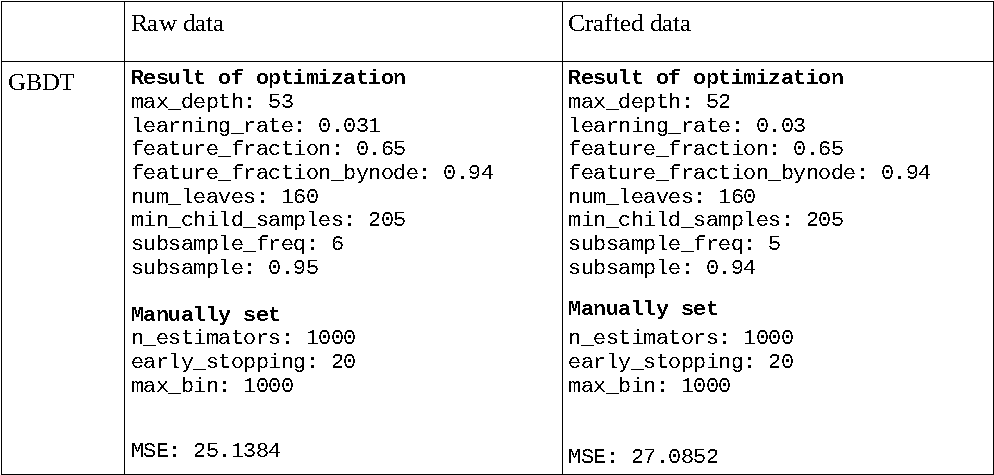
\includegraphics[width=\linewidth]{figures/HPO/GBDT_ResultsTable_HPO_Optimal.pdf}}
	\subfigure[Training history on data]{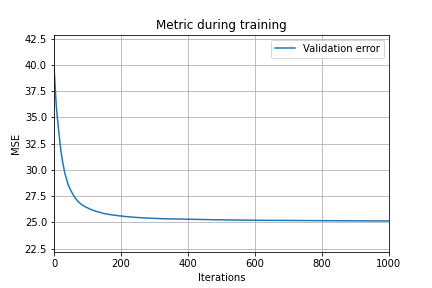
\includegraphics[width=0.49\linewidth]{../Implementation/optunaStudies/GBDT_Raw_Optimal.png}}
	\subfigure[Training history on crafted data data]{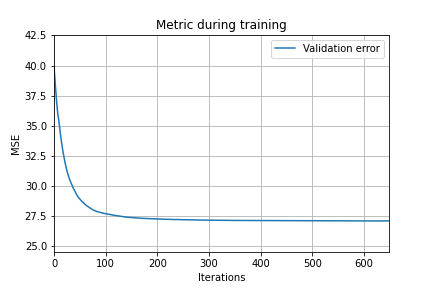
\includegraphics[width=0.49\linewidth]{../Implementation/optunaStudies/GBDT_Crafted_Optimal.png}}
	\caption{Optimal configurations and training history for GBDT}
	\label{fig:GBDT_Optimal}
\end{figure}
Figure \ref{fig:GBDT_ParallelPlot} depicts the parameter configurations of each optimization epoch in form of a parallel coordinate plot for GBDT on raw data in panel (a) and on crafted data in panel (b). Except the vertical gray line one the very left in the plots, each vertical gray axis represents the values ranging within the defined intervall of its corresponding parameter, whereas the very left line represents the axis for the objective values. The lines connecting all the parameter axes represent the parameter configurations of the optimization epochs. The bluer a line, the better the objective value - in our case the mean squared error. 
At first glance, it can be seen directly that the parameter configurations of both plots for good predictive performance are quite similar. For both sets, the mean squared error is minimized when we roughly use two-thirds of the features for each GBDT iteration (feature\_fraction, feature\_fraction\_bynode). Less test error is more likely achieved when we allow the algorithm to build rather deep trees up to a maximal depth of 50 while constraining the tree splitting process by specifying a lower bound of around 200 for the minimal amount of samples a node must contain in order to split it further (min\_child\_samples). We can furthermore see that a better objective value is attained when using nearly all samples considered for a GBDT iteration rather than applying (subsampling) and learning rates ranging between 0.03 to 0.05 (learning\_rate).

\begin{figure}[h]
	\centering
	\subfigure[On raw data]{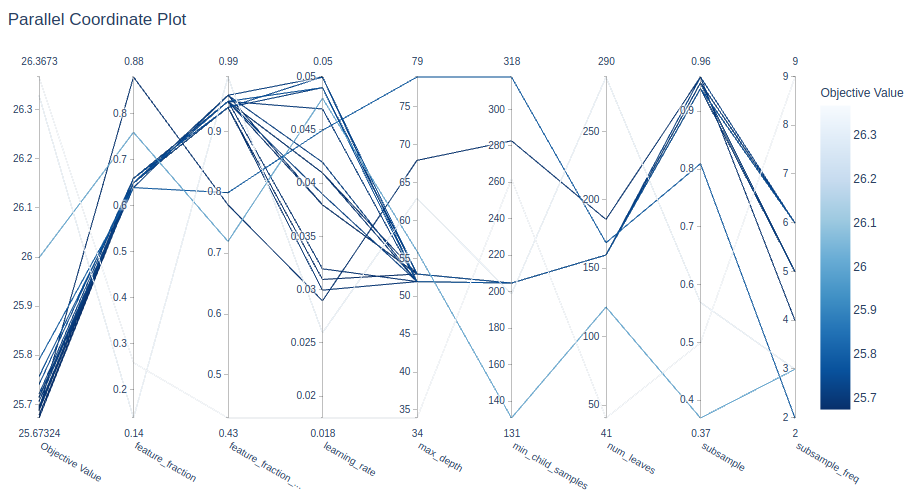
\includegraphics[width=\linewidth]{figures/HPO/GBDT_HPO_Raw_ParallelPlot.png}}
	\subfigure[On crafted data]{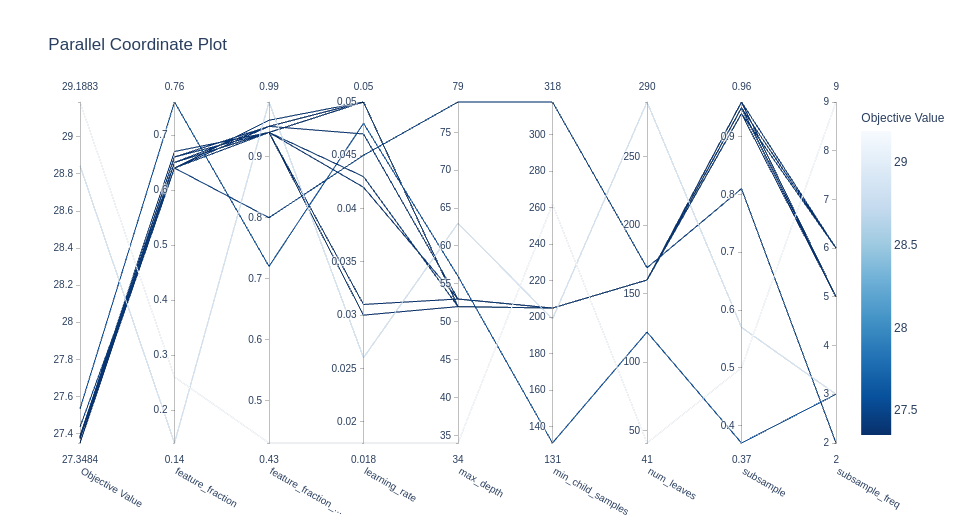
\includegraphics[width=\linewidth]{figures/HPO/GBDT_HPO_Crafted_ParallelPlot.png}}
	\caption{Parallel Coordinate Plots for GBDT}
	\label{fig:GBDT_ParallelPlot}
\end{figure}

Up next are the hyperparameter importances of GBDT depicted in figure \ref{fig:GBDT_Importances}. Panel (a) shows the importances for GBDT when trained on raw data
Panel (b) shows the importances for GBDT when trained on crafted data.
The x-axis of the importance plots depicts the relative parameter importances. 
On the y-axis is categorical and shows the parameters we considered to optimize. 
We can observe that the results for the datasets GBDT was trained on differ significantly. 
For GBDT on the raw data, we observe that choosing the right amount for subsampling, a suitable learning rate for calculating the gradient in GBDT, and the right feature fraction are of highest importance. For GBDT on the crafted data, we observe that the learning rate and the feature fractio are of even more relative importance, whereas the parameter for subsampling has far less significant impact on the objective value as compared to GBDT on raw data. 
We observe further non-trivial differences (here: $ \geq 5\%$ ) in relative importance for the subsampling frequency showing a difference 7\%, and for \textit{min\_child\_samples} with a difference of 5\%. For both datasets, the number of leaves, the percentage of features fractioned per node, and the maximal depth constraint for the estimators remain nearly equally important.   
\begin{figure}[h]
	\centering
	\subfigure[On raw data]{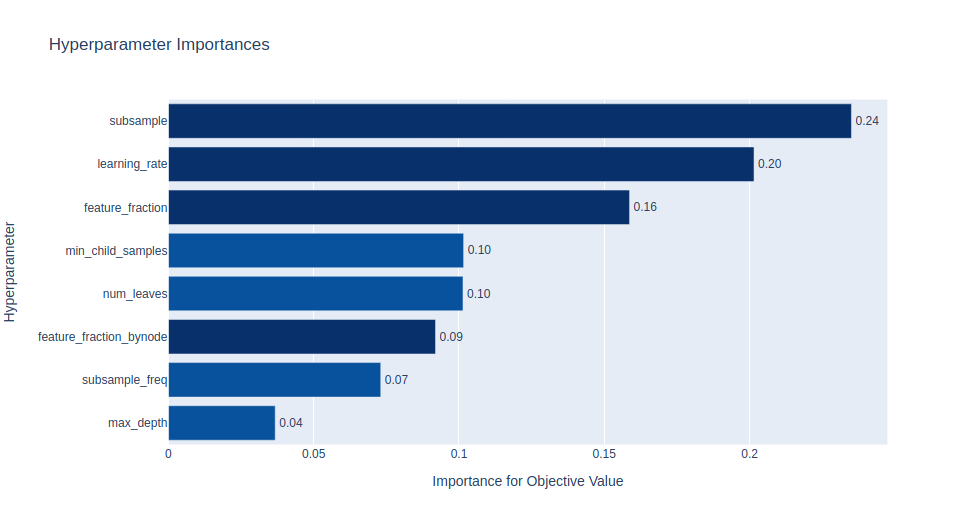
\includegraphics[width=\linewidth]{figures/HPO/GBDT_HPO_Raw_Importances.png}}
	\subfigure[On crafted data]{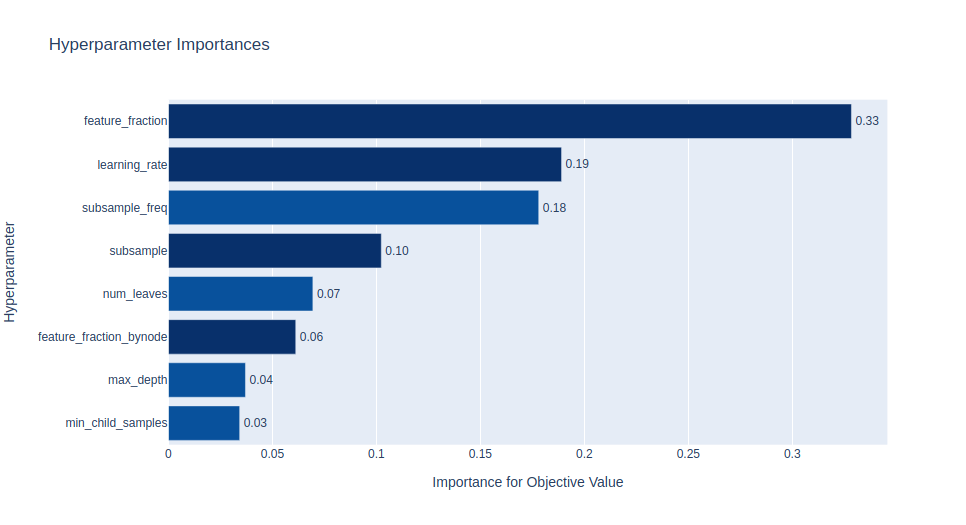
\includegraphics[width=\linewidth]{figures/HPO/GBDT_HPO_Crafted_Importances.png}}
	\caption{Hyperparameter Importances for GBDT}
	\label{fig:GBDT_Importances}
\end{figure}

Although there are significant differences between the hyperparameter importances for both GBDT experiment instances, the resulting optimal configuration of both does hardly differ as we have already pointed out. Thereby, we suggest that the difference in relative parameter importances does not affect the outcome of the optimization. We also suggest that the importances depend on the features that are used. We further found that the raw set achieves significant less test error than the crafted data set. This could be due to the reason that, besides the maximal time shift features, our raw set includes exactly any routing information of a customer's route that the state space of the RMDPEAT contains, whereas the crafted set includes only the amount of total stops, pick-up stops, and delivery stops. 
\clearpage
\subsection{Random Forest}
In this subsection, we will conduct HPO experiments for Random Forest on both datasets. 
For Random Forest, we decided to optimize following parameters and set the search spaces for each of them as follows:
\begin{description}[font=$\bullet$\scshape\bfseries]
	\item $ \text{max\_depth} \in [5, 100] $ in steps of 1.
	\item $ \text{feature\_fraction} \in [0.3, 1.0] $ in steps of 0.01.
	\item $ \text{feature\_fraction\_bynode} \in [0.3, 1.0] $ in steps of 0.01
	\item $ \text{num\_leaves} \in [900, 1200] $ in steps of 1
	\item $ \text{subsample\_freq} \in [1, 10] $ in steps of 1.
	\item $ \text{subsample} \in [0.3, 0.99] $ in steps of 0.01.
\end{description}
Besides the parameters considered for optimization, we set the number of estimators for one iteration in Random Forest to 1000 and enable early stopping with a patience of 20 as we did for the GBDT optimization. Additionally, we set \textit{min\_child\_samples} to 1 and thus exclude it from the set of parameters considered for optimization, because we found by trial-and-error that \textit{lightgbm-RF} performs best when it is set very low. We further set the parameter \textit{min\_data\_in\_bin} to 1 as we have again found by trial-and-error that this works well for \textit{lightgbm-RF}. Again, We are going to analyze optimal configurations with the help of the corresponding parallel plots first and then examine the hyperparameter importances for Random Forest for each dataset. 

Figure \ref{fig:RF_Optimal} depicts the optimal parameter configurations resulting of the HPO for the considered parameters and the respective training histories. Again, we observe that Random Forest on the raw data returns a lower test error of 26.5538 compared to the crafted features with a mean squared error of 27.7938 when trained on their respective optimal parameter configurations. Early Stopping sets in at around 170 iterations for the raw data instance, and at roughly 70 for the crafted data experiment instance. 
\begin{figure}[h]
	\centering
	\subfigure[Optimal configurations]{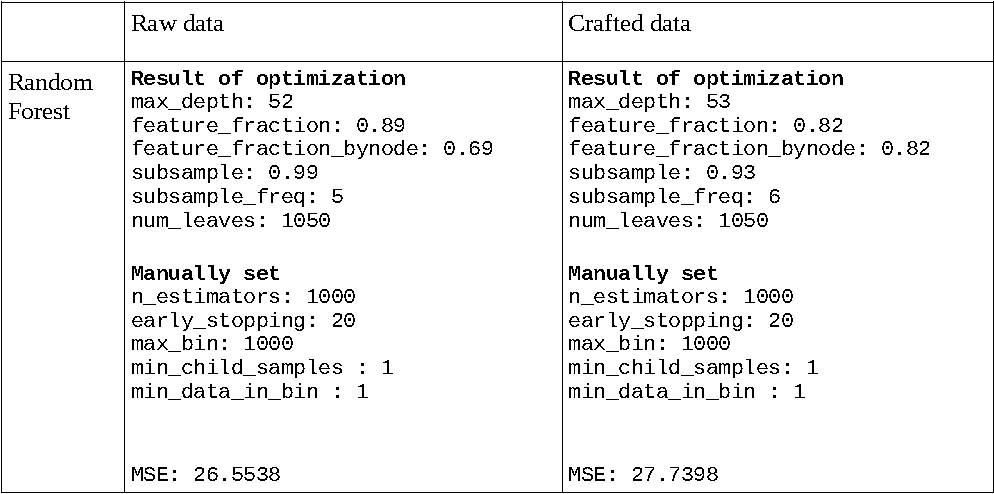
\includegraphics[width=\linewidth]{figures/HPO/RF_ResultsTable_HPO_Optimal.pdf}}
	\subfigure[Training history on raw data]{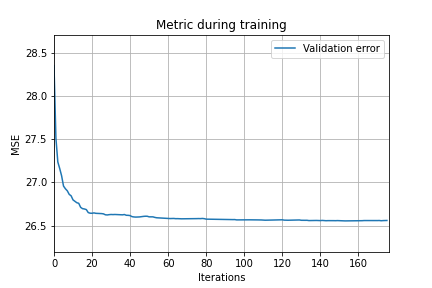
\includegraphics[width=0.49\linewidth]{../Implementation/optunaStudies/RF_Raw_Optimal.png}}
	\subfigure[Training history on crafted data]{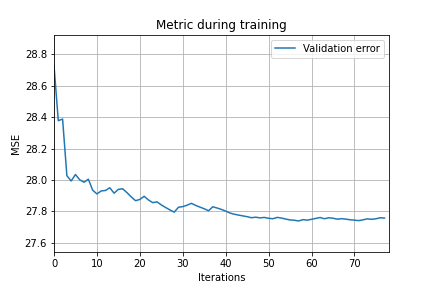
\includegraphics[width=0.49\linewidth]{../Implementation/optunaStudies/RF_Crafted_Optimal.png}}
	\caption{Optimal configurations and training history for Random Forest}
	\label{fig:RF_Optimal}
\end{figure}
Figure \ref{fig:RF_ParallelPlot} depicts the parallel coordinate plots for Random Forest on the raw and crafted features in panel (a) and (b) respectively. We observe that the distribution of parameter configurations achieving a comparably well objective value, is quite similar. A minimized objective value is achieved when the feature fraction and the feature fraction by node used for each estimator range between 0.8 and 1. Further, the maximal depth constraint set at a rather high value ranging between 50 and 60 seems to be optimal according to the HPO. The number of leaves each estimator has at the end of the iteration lies at roughly 1050 in most optimal cases. For subsampling, we observe that subsampling fraction greater than 90\% in a frequency of 6 goes is correlated to a minimized test error.
\begin{figure}[h]
	\centering
	\subfigure[On raw data]{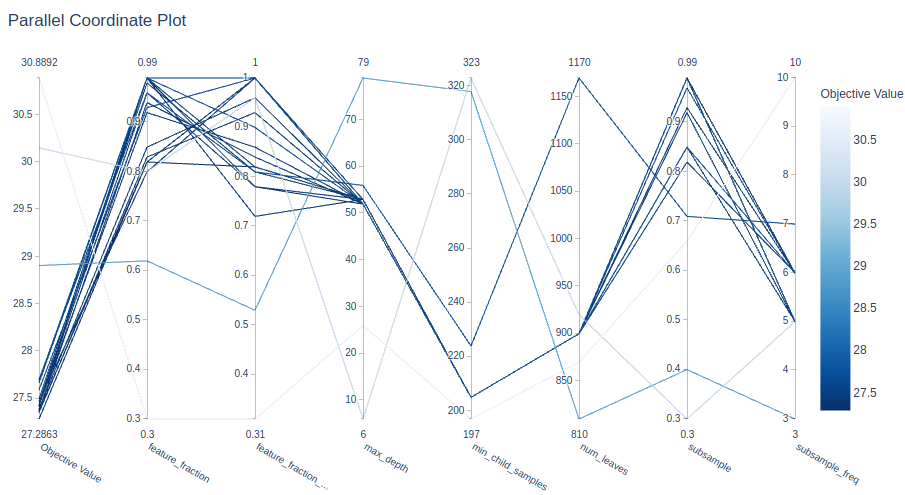
\includegraphics[width=\linewidth]{figures/HPO/RF_HPO_Raw_ParallelPlot.png}}
	\subfigure[On crafted data]{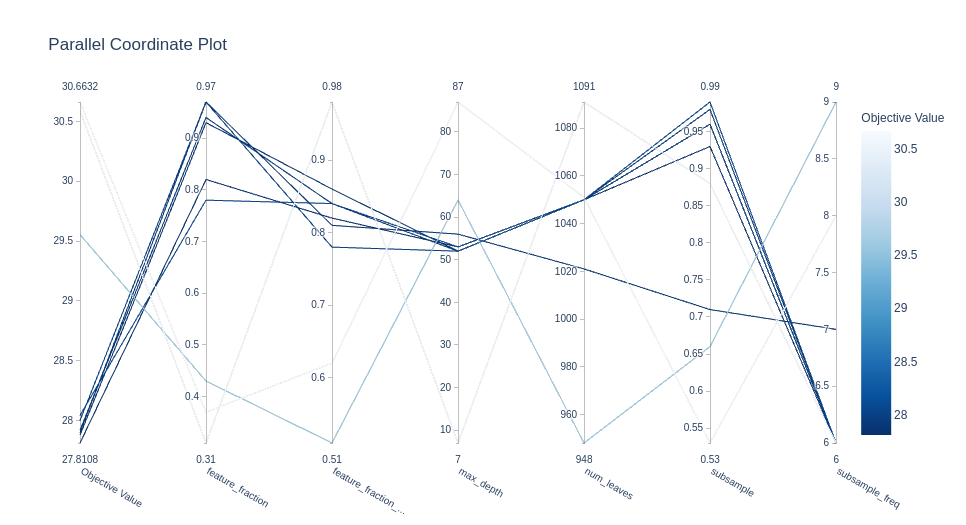
\includegraphics[width=\linewidth]{figures/HPO/RF_HPO_Crafted_ParallelPlot.png}}
	\caption{Parallel Coordinate Plots for Random Forest}
	\label{fig:RF_ParallelPlot}
\end{figure}

The hyperparameter importances for Random Forest on the raw and the crafted data are depicted in \ref{fig:RF_Importances}. For both instances, we observe that the chosen feature fraction has by far the most impact with a relative importance of 0.43 for the raw data instance, and 0.48 for the crafted data instance. Combining this information with the information given on the parallel plot, we conclude that it is crucial to set the feature fractions higher than 80\%. The instances significantly differ when it comes to subsampling and the subsampling frequence with differences of 10\% and 11\% respectively. When it comes to the maximum permitted depth and the number of leaves, the instances also show a percentual difference of 6\% and 3\% respectively.
\begin{figure}[h]
	\centering
	\subfigure[On raw data]{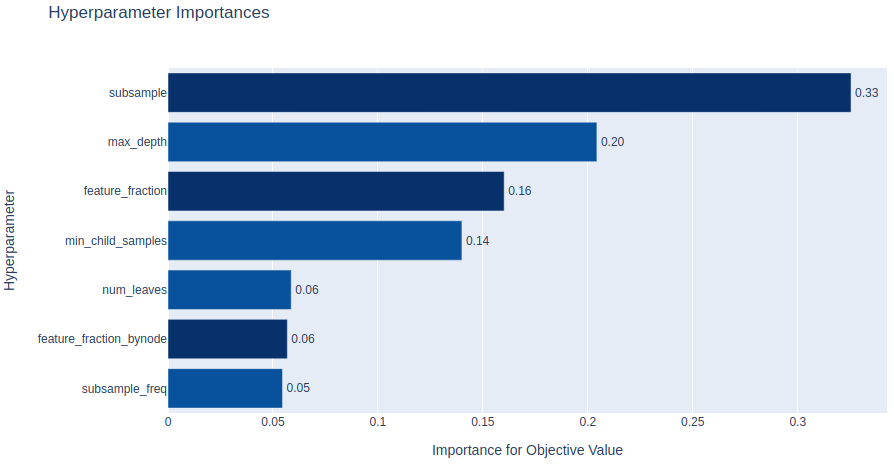
\includegraphics[width=\linewidth]{figures/HPO/RF_HPO_Raw_Importances.png}}
	\subfigure[On crafted data]{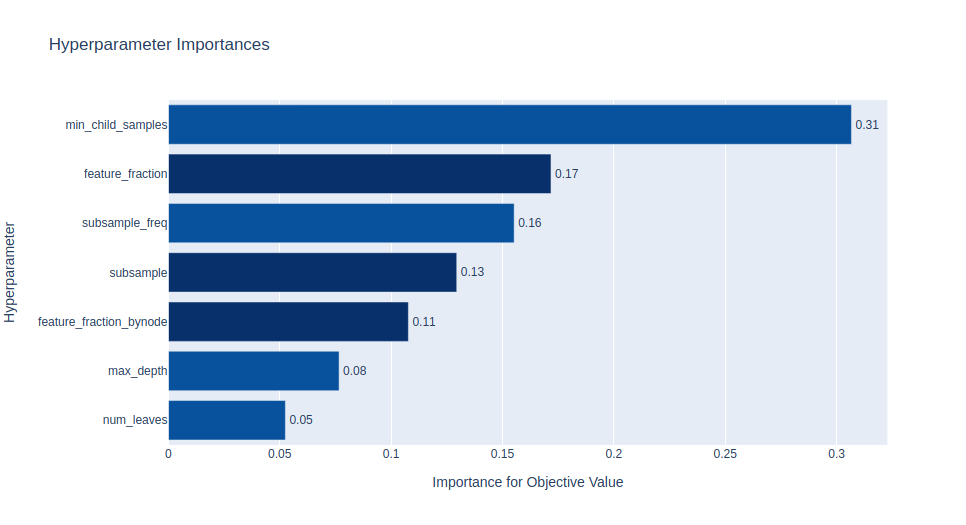
\includegraphics[width=\linewidth]{figures/HPO/RF_HPO_Crafted_Importances.png}}
	\caption{Hyperparameter Importances for Random Forest}
	\label{fig:RF_Importances}
\end{figure} 
 
\section{Experiment: Adding Noise}\label{sec:noise}







